\documentclass{sem5}
\usepackage{caption}
\institutename{Indian Institute of Information Technology, Vadodara}
\author{Dilip Puri}
\idt{201351014}
%\team{teamname}
\collab{\textbf{Collaborator} - Hemant Kumar(201352026)}

\coursename{Parallel Programming}
\ccode{\begin{small}CS403\end{small}}
\profname{Prof. Reshmi Mitra}

\type{Lab}
\typeid{03}
\submissiondate{\today}%dd/mm/yyyy
\deadline{Sep 5, 5:00 PM}%dd/mm/yyyy @hh:mm pm/am
\problemset{OpenMP(Open Multi-Processing)}

\begin{document}
\begin{enumerate}
\item Familiarize yourself with the OpenMP code given in this handout.
\item Using the command in the section on ``How to measure time for a block of C-code", find the time required in the thread function call in the previous lab assignment.\\
\begin{figure}[!htp]
\centering
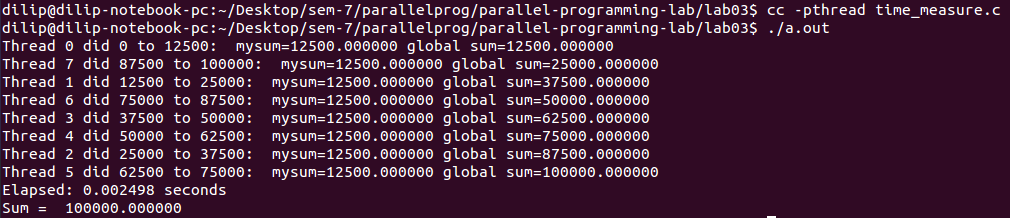
\includegraphics[scale=.4]{../2.png}
\caption{Elapsed time: 0.002498 seconds}
\end{figure}
\item Write a C-code using OpenMP threads to create an unbalanced load using sleep command and omp$\_$hello.c. The sample sleep times are given below:
\begin{enumerate}
\item thread-1: 10 sec, thread-2: 5 sec, thread-3: 20 sec, thread-4: 30 sec.
\item Measure the total time taken for the complete execution of code with and without the additional sleep command.\\
\begin{figure}[!htp]
\centering
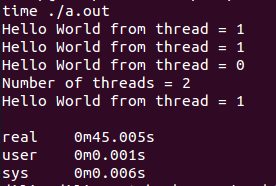
\includegraphics[scale=.6]{../31.png}
\caption{with sleep() command execution}
\end{figure}

\begin{figure}[!htp]
\centering
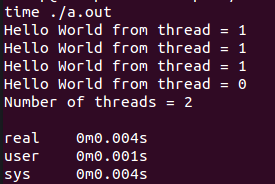
\includegraphics[scale=.6]{../32.png}
\caption{without sleep() command execution}
\end{figure}
\end{enumerate}

\item Write a threaded code using OpenMP on matrix multiplication:
\begin{enumerate}
\item Take overall execution time measurement using time command for different application size and thread count for the serial and parallel code.
\begin{center}
\captionof{table}{Execution Time}
\begin{tabular}{|l|c|c|c|c|c|c|}
\hline
Application Size & p=1 & p=2 & p=4 & p=8 & p=16 & p=32\\
\hline
5x5 & 0.000004&0.000009&0.000050&0.000115&0.000317&0.000484\\
\hline
10x10 &0.000017 &0.000021&0.000082&0.000236&0.000263&0.000416\\
\hline
100x100 & 0.015396&0.026991&0.027809&0.021341&0.021806&0.027567\\
\hline
500x500 &  0.674168&0.787767&1.368984&1.394844&1.349535&1.441614\\
\hline
1000x1000 &7.558727 &6.348322&15.236813&14.245590&14.108841&14.337918\\
\hline
\end{tabular}
\end{center}

\begin{center}
$Speedup = \frac{Execution Time(p)}{Execution Time(serial code)}$
\end{center}

\begin{center}
\captionof{table}{Speedup Time}
\begin{tabular}{|l|c|c|c|c|c|}
\hline
Application Size & p=2 & p=4 & p=8 & p=16 & p=32\\
\hline
5x5 & 2.25 & 12.5 & 28.75 & 79.25 & 121 \\
\hline
10x10 & 1.23 & 4.82 & 13.88 & 15.47 & 24.47\\
\hline
100x100 & 1.75 & 1.80 & 1.38 & 1.41 & 1.79\\
\hline
500x500 & 1.17 & 1.16 & 2.03 &  2.06 & 2.13 \\
\hline
1000x1000 & .84 & 2.01 & 1.88 & 1.86 & 1.90\\
\hline
\end{tabular}
\end{center}

\item Observe \texttt{gnome-system-monitor} output as your fire up different thread counts.\\
\begin{figure}[!htp]
\centering
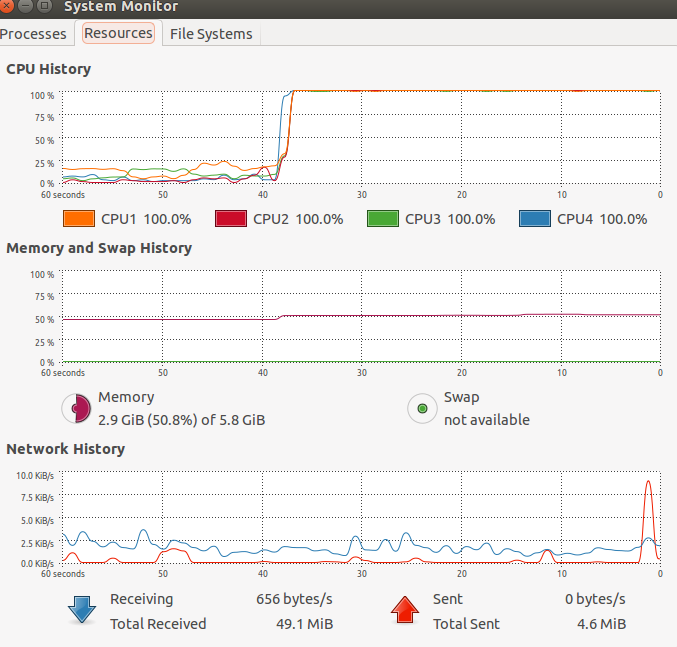
\includegraphics[scale=.3]{../t32.png}
\caption{for 32 threads 5000x5000}
\end{figure}
\item Use the overall execution time measurements to plot and comment upon the speed-up. Verify that:
\begin{enumerate}
\item Parallel execution time is more compared to the serial time when the application size is small.
\item For large application size, initially the speedup increases as you increase the number of threads. However, for very large number of threads (e.g. 64 threads) your performance becomes much worse w.r.t. serial code and lower thread count.

\end{enumerate}
\end{enumerate}

\item \textbf{Multi-access threaded queue - using OpenMP}
Implement a multi-access threaded queue with multiple threads inserting and multiple threads extracting from the queue. Use mutex-locks to synchronize access to this queue. Document the time for 1000 insertion and 1000 extractions each with 4 insertion threads (producers) and 4 extraction threads (consumers).(Buffer size = 250)
\end{enumerate}

\begin{itemize}
\item[3] Multi-access threaded queue
\begin{enumerate}
\item Implement a multi-access threaded queue with multiple threads inserting and multiple threads extracting from the queue. Use mutex-locks to synchronize access to this queue. Document the time for 1000 insertion and 1000 extractions each with 4 insertion threads (producers) and 4 extraction threads (consumers).

\item Repeat above problem with condition variables (in addition to mutex locks). Document the time for the same test case as above. Comment on the difference in the times.

\end{enumerate}
\end{itemize}
\end{document}